% !TeX root = ../main.tex
% !TEX root = ../main.tex
% -*- root: ../main.tex -*-
% -*- program: pdflatex -*-
\chapter{~MRPC~端盖~TOF~离线数据}
原来的端盖~TOF~采用的塑料闪烁体,分东西两部分,每部分单层结构,闪烁体为扇形,光电倍增管垂直耦合,放置于扇形闪烁体的内端。每部分有~48~块。
图~\ref{fig:end-TOF-sigma}~给出了~ETOF~的时间分辨。
对于双~$\mu$子~事例样本,时间分辨为~110ps~,~Bhabha~事例中,时间分辨为增至~148ps~\cite{zhaoc:2011}。分辨率的差异主要来自不同粒子与实
验装置材料不同作用的差别,由于~$\mu$~散射最小,击中塑料闪烁体的位置不确定性较小,相比较~Bhabha~中的电子事例而言(由于位置的不确定性以及多次散射)非本征的时间分辨贡献小,因而时间分辨较好。
\begin{figure}[!h]
  \centering
  \includegraphics[width=0.9\textwidth]{chap1/end-TOF-sigma.png}
  \caption{端盖ETOF 的时间分辨:(a)电子和(b)~$\mu$~子}
  \label{fig:end-TOF-sigma}
\end{figure}
图~\ref{fig:end-TOF-eff}~给出了~ETOF~的各探测单元的效率。探测效率大致为~96$\%$~\cite{wangxz2016}。
\begin{figure}[!h]
  \centering
  \includegraphics[width=0.8\textwidth]{chap1/end-TOF-eff.png}
  \caption{端盖ETOF 的各探测器单元的效率}
  \label{fig:end-TOF-eff}
\end{figure}

对于~ETOF~而言,由于多次击中粒子,导致性能相比桶部明显较差。~ETOF~的~$\pi/K$~的分辨能力如图~\ref{fig:end-TOF-PID}~\cite{zhaoc:2011}所示,在~95.4$\%$(2$\sigma$)~正确率下,基本满足动量~1.1GeV~以内的~$\pi/K$~介子的鉴别。

\begin{figure}[!h]
  \centering
  \includegraphics[width=0.9\textwidth]{chap1/end-TOF-PID.png}
  \caption{~1.0Gev~下$\pi$~(a)和~$K$~(b)的时间分辨;(c):端盖~ETOF~不同角度下的$\pi/K$ 分辨}
  \label{fig:end-TOF-PID}
\end{figure}

相比于桶部~TOF~(双层闪烁体)的性能指标,~BESIII~端盖~TOF~,由于端盖~TOF~是单层闪烁体,以及端盖部分多次散射的影响较大,其本征时间分辨和非本征时间分辨都比较大。

BESIII~谱仪的设计目标是在~$\tau$-粲能区的高精度测量,在这一能区~$J/\psi$~衰变是最主要的物理过程。模拟结果显示,~$J/\psi$~衰变强子动量分布可以达到~1.5GeV/c~,虽然在~0.95GeV/c~以上的强子占的比例较小,但是,对于~BES~物理追求的高精度测量以及稀有衰变事例的研究仍然是非常重要的。因此进一步提高其粒子鉴别能力, 对于提升整个谱仪粒子鉴别能力,完成~BES~物理目标具有重要意义。

测量中性D介子系统的CP破坏和混合参数是~BESIII~的物理目标之一。D介子是唯一没有被测量到CP破坏的重味介子。测量D介子混合的黄金衰变道是~$D^0 \to K^- \pi^+$~,~$D^0 \to K^- \pi^+\pi^-\pi^+$~,~$D^+ \to K^- \pi^+\pi^+$~
由于$K$和$\pi$介子的动量分布在~0.8-1.05GeV,这样我们需要很好的~$\pi/K$~粒子鉴别,要达到较显著的测量结果,要求~$\pi/K$~误鉴别率在~1.05GeV~时要达到~1$\%$~以下。

而~BESIII~目前的端盖~TOF~时间分辨为~140ps, ~$\pi/K$~的误鉴别率在~1.05GeV~时约为~5$\%$~左右,使得中性D介子的混合参数测量显著性很大程度上下降。由于D介子系统的CP破坏很小,粒子物理的标准模型预言CP破坏的大小在千分之一左右,要求测量的寻迹系统误差很小,同时也要求~$\pi/K$~的误鉴别应该在~1$\%$~以下。端盖~TOF~的改造不仅改善对带电径迹的粒子鉴别,同时好的飞行时间测量也能提高主漂移室对带电径迹的测量精度,改善寻迹的系统误差,特别是端盖小角度的误差和误鉴别率的改善。当然对于D介子的半轻子衰变和形状因子以及CKM矩阵元Vcs和Vcd的测量,改造后的~TOF~端盖会降低由于粒子误鉴别造成的本底,提高这些物理量的测量精度。 

\section{MRPC硬件和电子学}
\subsection{端盖MRPC的结构}
升级后的端盖~TOF~采用了MRPC技术。利用~MRPC~做成的飞行时间探测器有好的时间分辨,同时又能保证探测效率,有高的粒子鉴别能力,而且价格也便宜。从~MRPC~探测原理分析,当带电粒子穿过~MRPC~时,其原初电离的雪崩放大过程是在多个气隙中进行,因此气隙的宽度与数目是决定~MRPC~性能的重要的参数。采用较小的气隙宽度可以降低工作电压提高工作稳定性;增加气隙数目,由于增加了带电粒子在气隙中产生雪崩的几率,可以提高其探测效率;减小了雪崩过程的统计涨落有利于提高时间分辨。

采用MRPC的端盖TOF的具体阵列设计如图~\ref{fig:MRPC-TOF}~所示,每层18个模块,采用双层结构,通过相邻模块间的交叠可以减少死区,提高探测效率。
\begin{figure}[!h]
  \centering
  \includegraphics[width=0.5\textwidth]{chap1/MRPC-TOF.png}
  \caption{BESIII/ETOF 双层MRPC阵列结构示意图}
  \label{fig:MRPC-TOF}
\end{figure}

每个模块的PCB的设计如图~\ref{fig:PCB}~所示。每个模块采用梯形结构,共有12个读数条,读数条宽2.4cm,相邻读数条之间的距离为3mm。读数条最短的是9.1cm,最长的是15.1cm。每个读数条采用双端读出,共有24路读出信号通道。

\begin{figure}[!h]
  \centering
  \includegraphics[width=0.9\textwidth]{chap1/PCB.png}
  \caption{MRPC结构示意图}
  \label{fig:PCB}
\end{figure}

MRPC模型几何结构如图~\ref{fig:MRPC}~所示。模块采用双层堆叠的设计方式,一共2*6个气隙,每个气隙220 $\mu$m,每个模块的厚度$<$2.4cm, 双层总厚度$<$5cm;环状探测器外半径为844mm,内半径为454mm。
\begin{figure}[!h]
  \centering
  \includegraphics[width=0.9\textwidth]{chap1/MRPC.png}
  \caption{ETOF 升级MRPC 的结构图}
  \label{fig:MRPC}
\end{figure}

MRPC~需要工作在气密的环境下,工作气体组分是90$\%$~Freon+5$\%$~S$F_{6}$+5$\%$~iso-$C_{4}H_{10}$。
\subsection{电子学系统}

MRPC的电子学系统设计方案和电子学系统包含前端放大甄别FEE(Front end Electronics)模块、飞行时间测量TDIG(Time to Digital module)插件、提供阈值和电源给FEE模块并传输击中信息至触发系统等功能的CTTP (Coincidence Test Threshold Power module)插件,时钟扇出插件硬件系统和数据获取软件和控制软件系统。

整个系统共72个FEE模块,FEE模块采用基于TOT技术的NINO芯片,每个FEE模块含有4片NINO芯片,产生24路LVDS电平的输出信号,共完成1728路信号的放大甄别。
MRPC输出电荷约为几十fC, 脉冲上升时间$<$1ns,实验上必须对输出信号电流进一步放大和成形。~NINO-ASIC~芯片采用差分的输入,全线路的差分信号处理,最大程度的利用了~MRPC~本身产生的差分信号。NINO~对输入信号进行快放大,同时~NINO~ 将输入的信号电流转换为输出的信号宽度,以满足~TOT~测量的需要。
飞行时间数字化插件TDIG。使用HPTDC芯片,接收和数字化前端电子学输出的信号并根据数据格式打包,经VME总线上传至DAQ系统。~NINO~配合~HPTDC~同时测量出信号过阈时间的前沿时间(leading edge)和后沿时间(trailing edge)。其中前沿时间用来定时,结合前沿时间和后沿时间的~TOT~用来修正过阈时间不同引起的时间晃动。
ETOF电子学系统中,CTTP插件共两块,一个CTTP插件对应36个FEE模块。插件接收NINO芯片产生的击中信息,通过光纤上传至触发系统;为NINO芯片提供阈值电压,电源和测试信号,使芯片正常运行和满足测试需求。CTTP插件同时还完成快控制功能。
时钟扇出插件为TDIG和CTTP插件提供同步时钟信号。

\section{BESIII离线数据处理和分析系统}
BESIII~离线数据处理和分析系统是为~BESIII~实验开发的全新软件系统,包括软件平台、模拟、刻度、重建和物理分析工具等部分。它的主要任务是将探测器和模拟产生的原始数据进行离线处理,生成物理分析使用的包含末态粒子各种信息的数据(DST数据),同时提供物理研究需要的各种软件工具,是连接物理分析和探测器的桥梁。~BESIII~的简化的离线数据处理过程如图~\ref{fig:BESIII-data-flow}~所示。
\begin{figure}[!h]
  \centering
  \includegraphics[width=0.9\textwidth]{chap1/BESIII-data-flow.png}
  \caption{简化的BESIII离线数据处理和物理分析过程}
  \label{fig:BESIII-data-flow}
\end{figure}

离线数据处理和分析软件平台~\cite{liwd:2006}(BOSS)是BESIII离线软件系统的核心。~BOSS~是以欧洲核子中心~LHCb~实验开发的通用高能物理实验底层软件~GAUDI~~\cite{Barrand:2000}为基础,根据~BESIII~实验的具体需求,以C++语言为主开发的全新离线数据处理软件。

BOSS软件平台可以为包括离线刻度、事例重建、事例分类、蒙特卡罗模拟和物理分析等阶段的离线数据处理提供有效的数据管理工具。软件平台根据数据处理各阶段的特点,设计了符合探测器特点的数据结构,然后利用专门的数据管理服务对这些数据进行管理。BOSS软件平台实现动态库的链接机制,可以有效的缩短再编译的时间。软件系统也采用了国际高能物理实验室的开源软件库和各种工具软件,如ROOT~\cite{root},CERNLIB~\cite{cern}等。


图~\ref{fig:BESIII-software}给出了BESIII离线软件平台的整体结构图。其中的模拟、刻度、重建和物理分析算法是离线数据处理和物理分析的核心。
\begin{figure}[!h]
  \centering
  \includegraphics[width=0.9\textwidth]{chap1/BESIII-data-flow.png}
  \caption{BESIII离线软件平台}
  \label{fig:BESIII-software}
\end{figure}

BESIII数据处理和物理分析软件系统包含超过200个软件单元,采用软件包的形式来组织和管理软件。BESIII采用配置管理工具(Configuration Management Tool,CMT)来规范软件开发和发布过程,并且为该过程提供一套完整的配置管理工具。%【9】

\section{端盖TOF数据刻度重建流程}
BESIII~离线事例重建软件系统由MDC、EMC、TOF和MUC子系统以及径迹外推和匹配部分组成。BEPCII~采用了多束团对撞机制,每个束团的时间间隔为6ns,而BESIII触发系统的工作周期为24ns,即每个触发周期内有4个束团对撞。因此每个事例产生的准确时间不能有在线系统直接给出,必须通过离线软件通过事例重建,主要是MDC径迹重建,寻找最可几事例起始时间。

事例重建系统的一般流程如图~\ref{fig:reconstruction}~。

\begin{figure}[!h]
  \centering
  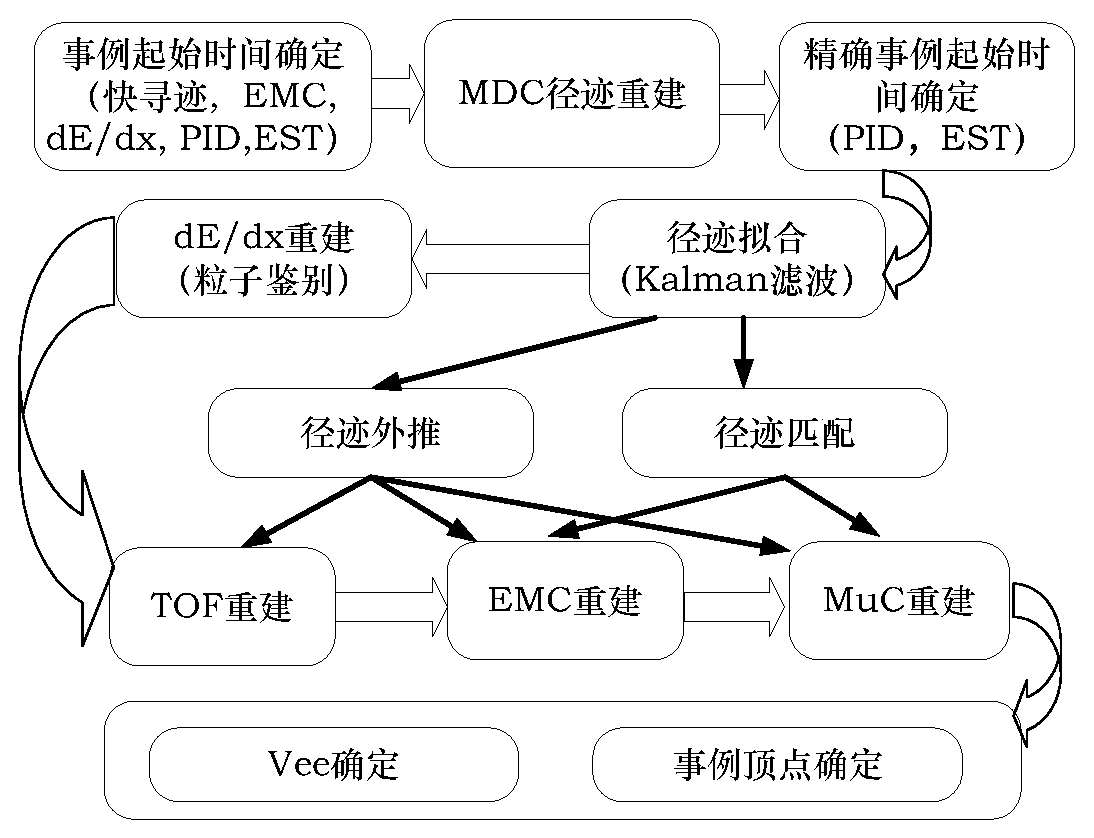
\includegraphics[width=0.7\textwidth]{chap1/reconstruction.eps}
  \caption{BESIII事例重建过程}
  \label{fig:reconstruction}
\end{figure}

\subsection{事例起始时间重建}

BEPCII采用多束团对撞机制,BEPCII的高频时钟为499.8MHz,周期为2ns,储存环中共有93个束团,每个束团之间的时间间隔为6ns。BESIII触发系统的周期为24ns,因此每个触发周期内有4个束团对撞,准确的事例起始时间无法由在线系统给出。图~\ref{fig:BESIII-time-system}给出了BESIII的时间测量系统。事例的起始时间$T_{est}$可以表示为:$T_{est}$=$T_{DCM}$-$T_{ev}$。其中$T_{est}$为事例起始时间,即实际对撞时刻与触发周期前沿时刻的时间差;$T_{DCM}$为电子学给出的TOF测量到的TDC时间,$T_{ev}$为粒子从对撞点到给出信号的探测器之间的飞行时间。
\begin{figure}[!h]
  \centering
  \includegraphics[width=0.6\textwidth]{chap1/BESIII-time-system.png}
  \caption{BESIII事例的时间关系}
  \label{fig:BESIII-time-system}
\end{figure}

图~\ref{fig:Test}~给出了计算事例起始时间$T_{est}$的程序流程图。主要包括快重建~\cite{zhangxm:2005}和时间起始时间重建两部分~\cite{max:2007}。在MDC快重建和粒子鉴别完成后,$T_{est}$由~MDC~和~TOF~分别计算得到,具体的计算方法见文献~\cite{Maxiang:2008}。其中TOF得到的$T_{est}$精确度高。

\begin{figure}[!h]
  \centering
  \includegraphics[width=0.6\textwidth]{chap1/Test.png}
  \caption{事例起始时间程序流程图}
  \label{fig:Test}
\end{figure}
\subsection{MDC的径迹外推}

~BESIII~主漂移室重建径迹的外推算法采用面向对象的设计方法, 利用~GEANT4~部分代码开发实现, 它提供主漂移室带电径迹外推到外部其他子探测器上的预期径迹信息。该算法的外推过程考虑了带电径迹在磁场中的偏转以及与探测器物质相互作用造成的电离能损, 并为径迹参数计算考虑了库仑多次散射效应影响在内的参数误差矩阵.

在考虑带电粒子的磁场偏转、电离能损的情况下较精确的计算径迹预期参数的一个常用方法是小步长外推. 该方法把径迹近似为螺旋线, 在每个小步长结束时从粒子动量中减去该步长的电离能损,然后再进行下一个小步外推, 直到推至要求的位置~\cite{wangll:2014}。
图~\ref{fig:TrkExtAlg}~给出了径迹外推程序~TrkExtAlg~流程图。

\begin{figure}[!h]
  \centering
  \includegraphics[width=0.6\textwidth]{chap1/TrkExtAlg.png}
  \caption{径迹外推算法的实现流程图}
  \label{fig:TrkExtAlg}
\end{figure}

\subsection{TOF重建}
TOF离线数据重建流程如图~\ref{fig:TOF-res}~所示。
TOF电子学系统给出TOF的时间信号和幅度信号。MDC重建和KalmanFilter径迹拟合得到带电径迹的动量和径迹长度等信息~\cite{wulh2007}~\cite{wangjk2009},进而计算出粒子飞行的预期时间,径迹外推给出击中TOF的位置信息~\cite{wangll:2014},事例起始时间算法~\cite{Maxiang:2008}给出$t_{0}$信息,利用这些信息结合刻度得到的刻度常数完成TOF的离线数据重建。
\begin{figure}[!h]
  \centering
  \includegraphics[width=0.6\textwidth]{chap1/TOF-res.png}
  \caption{TOF的离线数据重建过程}
  \label{fig:TOF-res}
\end{figure}

\section{原始数据分布?}
图~\ref{fig:digicheck-endcapLeading-east-endcap-histogram}~给出了MRPC端盖TOF的原始的TDC的信息。
\begin{figure}[!h]
  \centering
  \includegraphics[width=0.75\textwidth]{chap1/digicheck-endcapLeading-east-endcap-histogram.eps}
  \caption{原始的TDC}
  \label{fig:digicheck-endcapLeading-east-endcap-histogram}
\end{figure}

图~\ref{fig:T and Q}~给出了T-Q匹配后MRPC端盖TOF的原始的T和TOT的分布。
\begin{figure}[!h]
\begin{minipage}{0.48\linewidth}
  \centerline{ \centering \includegraphics[width=0.8\textwidth]{chap1/endcapcheck-east-t-histogram.eps}}
  \centerline{(a) 东端的原始时间}
  \centerline{\label{fig:endcapcheck-east-t-histogram}}
\end{minipage}
%\hfill
\begin{minipage}{0.48\linewidth}
  \centerline{ \centering 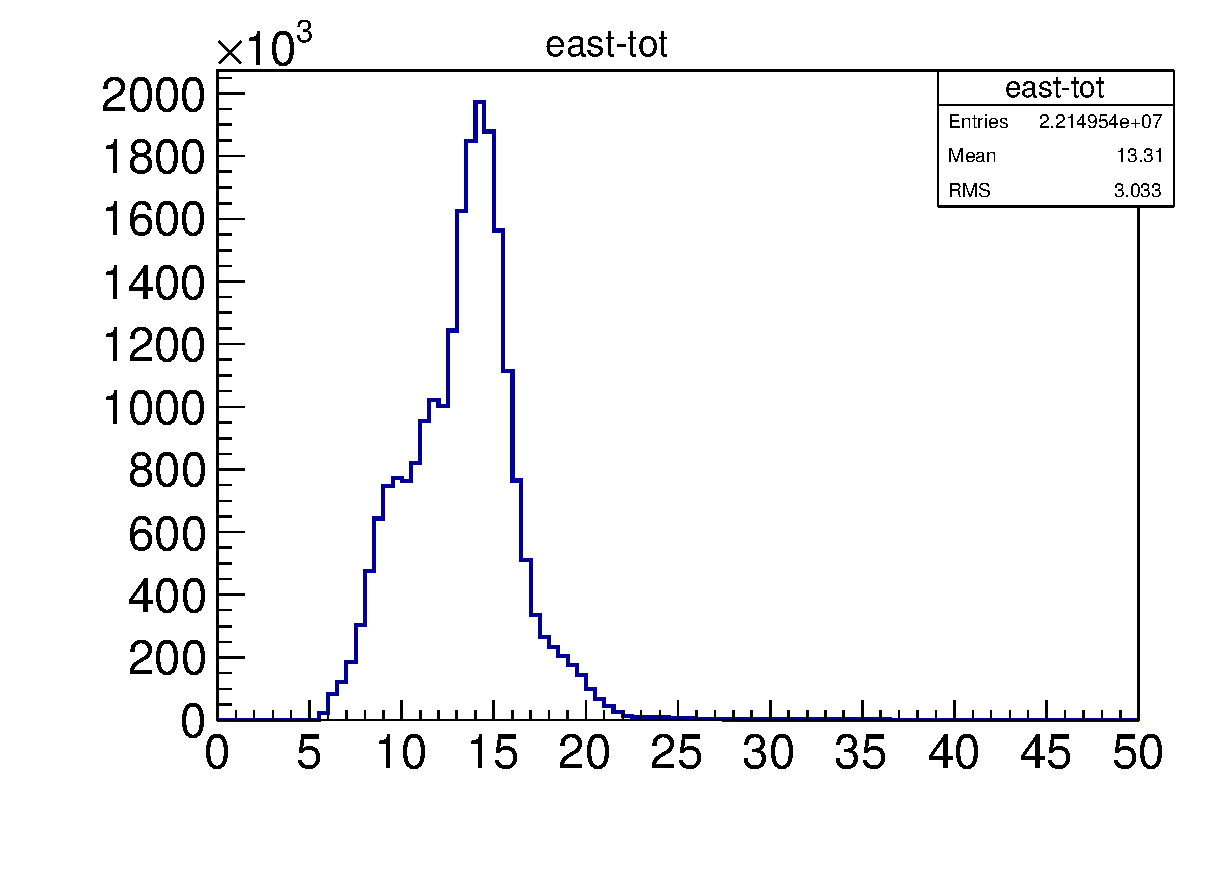
\includegraphics[width=0.8\textwidth]{chap1/endcapcheck-east-tot-histogram.eps}}
  \centerline{(b) 东端的原始TOT}
  \centerline{\label{fig:endcapcheck-east-tot-histogram}}
\end{minipage}
\vfill
\begin{minipage}{0.48\linewidth}
  \centerline{ \centering  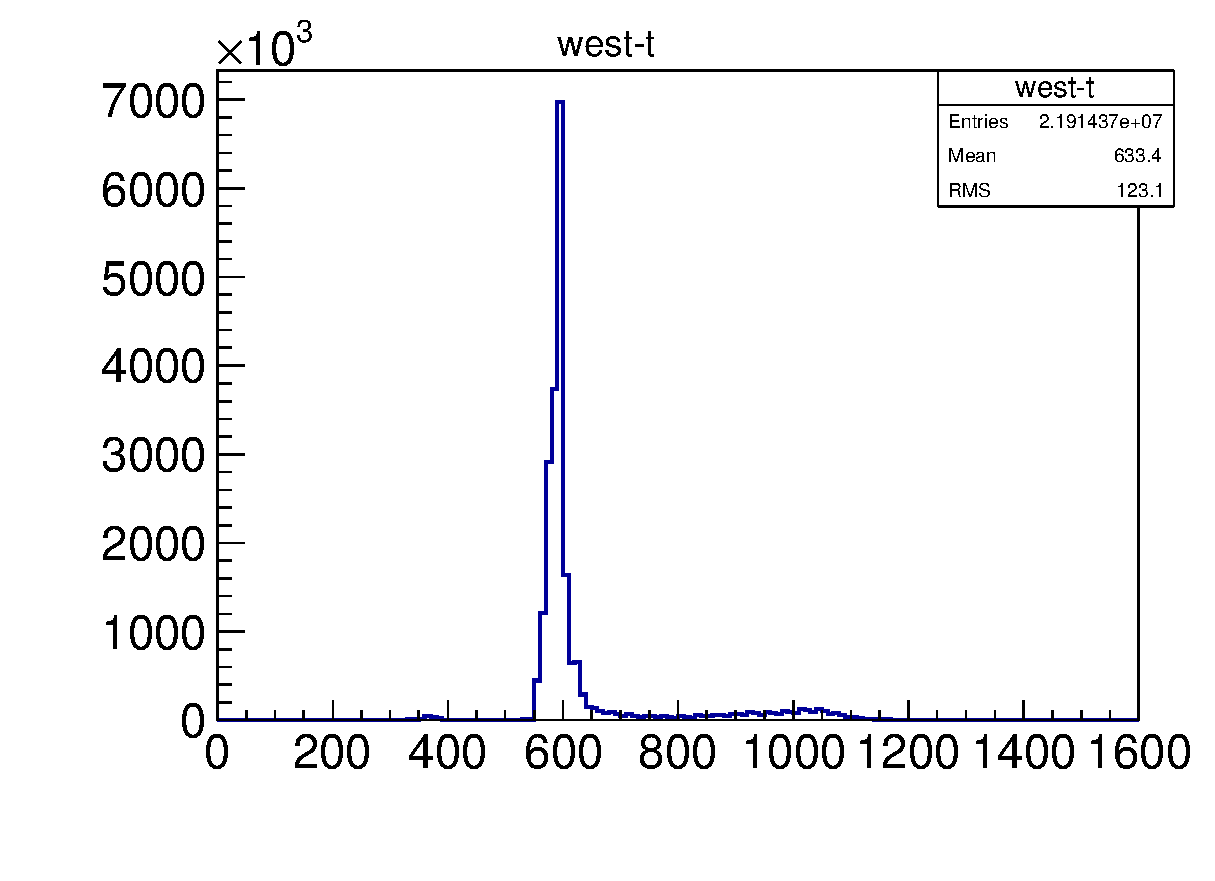
\includegraphics[width=0.8\textwidth]{chap1/endcapcheck-west-t-histogram.eps}}
  \centerline{(c) 西端的原始时间}
  \centerline{\label{fig:endcapcheck-west-t-histogram}}
\end{minipage}
%\hfill
\begin{minipage}{0.48\linewidth}
  \centerline{ \centering 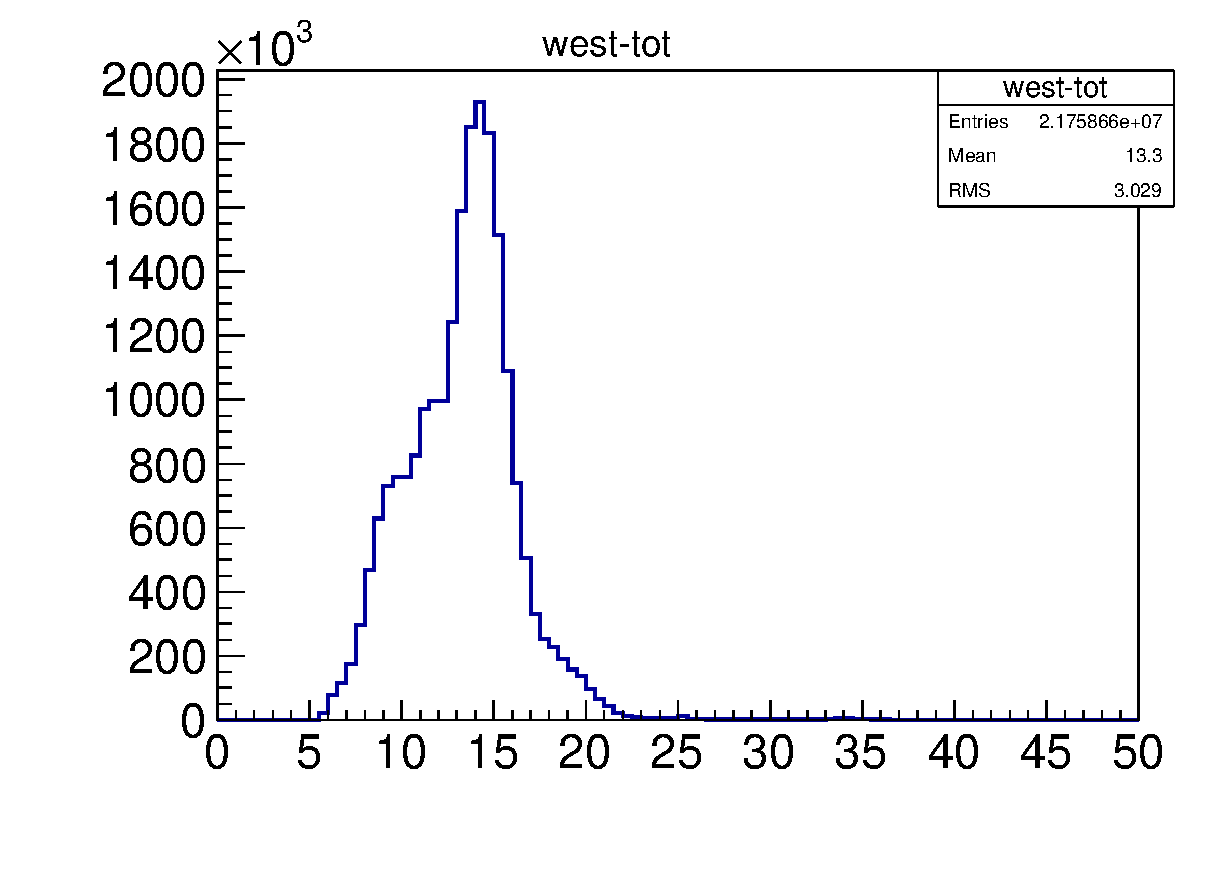
\includegraphics[width=0.8\textwidth]{chap1/endcapcheck-west-tot-histogram.eps}}
  \centerline{(d) 西端的原始TOT}
  \centerline{\label{fig:endcapcheck-west-tot-histogram}}
\end{minipage}
\caption{T-Q匹配后MRPC的原始时间和TOT的分布}
\label{fig:T and Q}
\end{figure}

图~\ref{fig:tofcheck-endcap-est-histogram}~给出了事例起始时间的分布。
\begin{figure}[!h]
  \centering
  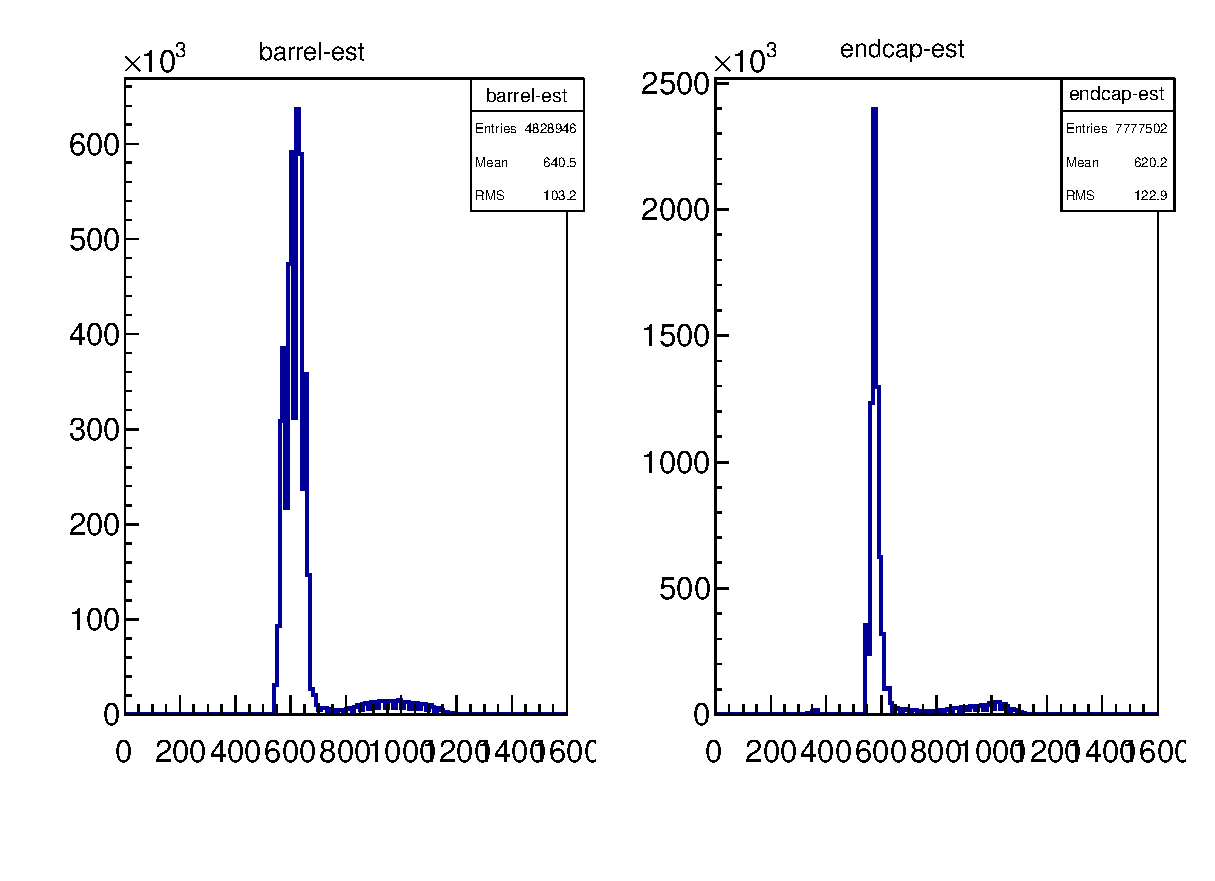
\includegraphics[width=0.75\textwidth]{chap1/tofcheck-endcap-est-histogram.eps}
  \caption{事例起始时间的分布}
  \label{fig:tofcheck-endcap-est-histogram}
\end{figure}

原始测量的时间信号TDC包括事例的起始时间~$t_{0}$~,对撞事例从对撞顶点到~TOF~探测器的飞行时间~$t_{tof}$~,信号在读数条的传播时间~$t_{pro}$~,电子学的延迟~$t_{ele}$~,过阈时间的晃动~$t_{time-walk}$~。即:~TDC=$t_{0}$+$t_{tof}$+$t_{pro}$+$_{ele}$+$t_{time-walk}$~,所以飞行时间~$t_{tof}$=TDC-($t_{0}$+$t_{pro}$+$_{ele}$+$t_{time-walk}$)~,其中TDC是TOF探测器测量到的原始时间信号,对于~MRPC~来讲,采用的双端读数,所以一个事例有两个~TDC~时间信号。~$t_{0}$~由事例起始时间算法给出,~$t_{pro}$~对于~MRPC~来说是信号在对数条的传播时间。这个是刻度的主要内容之一。~$t_{ele}$~是电子学延迟项,是一个常数项。~$t_{time-walk}$~对于MRPC来说是TOT的晃动。
\section{刻度的重点和难点}
\subsection{MRPC离线刻度的信息量}
前面已经介绍了MRPC直接测量的是时间信号TDC,还有过阈时间TOT。MRPC的读数条采用的是双端的读出形式。所以对应一个事例测量的有两个时间信号TDC1,TDC2;有两个过阈时间TOT1,TOT2。
在这里定义:
\begin{align}
tleft=TDC1-t_{0}
\label{eq:tleft}\\
tright=TDC2-t_{0}
\label{eq:2}
\end{align}
则tleft和tright为事例从对撞点时刻到电子学读出的过阈时间前沿的时刻之间的间隔。包括从对撞点飞行到MRPC探测器的飞行时间,信号在读数条中的传播时间,信号在电缆等的传播时间,电子学的时延,过阈时间的晃动等部分。

刻度的目的正是修正除了飞行时间外的其它时间的贡献。其中信号在电缆的传播时间和电子学的时延是常数项,信号在读数条的传播时间是一个依赖击中位置的时间量。过阈时间的晃动是和信号的大小有关的量。

BESIII系统的坐标定义为:正Z轴沿着束流方向,水平向东;正Y轴指向天空,竖直向上;正X轴取水平向北。取对撞点为坐标原点O(0,0,0)。空间某一点P(x,y,z)的方位角定义为直线OP从正X轴沿逆时针在Z—Y平面投影的角度$\phi$,在端盖~MRPC~中对应的不同模块的编号tofid和相同模块不同的击中位置~zrhit(来自径迹外推)。OP的极角定义为OP和正Z轴的夹角$cos\theta$,在端盖~MRPC~中对应的是读数条的编号~strip。

之前已经介绍了利用~MDC~重建和卡曼滤波径拟合可以得到带电径迹的动量和径迹长度的信息,进而可以求出带电粒子的预期飞行时间$t_{exp}$。

至此,刻度需要的所有相关量已经介绍完了。包括电子学系统测量的量:初始时间~tleft,tright~(TDC扣除$t_{0}$的时间在本论文中仍旧称为初始时间),过阈时间~qleft,qright~(测量的两个TOT的值在本文中都表示成~qleft,qright~的形式);外推的量:击中位置~zrhit,预期时间~$t_{exp}$,以及模块的编号~tofid,读数条的编号~strip。
\subsection{MRPC离线刻度的时间,TOT,zrhit等的原始分布}
图~\ref{fig:some-Diagram}~给出了MRPC离线刻度的一些原始的分布。上面的三幅图是原始的时间,过阈时间和击中位置分布的一维图,其中~\ref{fig:left-t}~是原始的时间tleft的分布;~\ref{fig:left-q}~是原始的过阈时间qleft的分布,可以明显看出,存在多峰现象;~\ref{fig:left-z}~是击中位置zrhit的分布,可以看出事例数随着zrhit是分布均匀的。下面三幅图是原始的时间,过阈时间和击中位置相互关系的二维图,其中~\ref{fig:left-tVSz}~表示时间随击中位置的分布,这个关系近似线性,这是刻度的主要项之一;~\ref{fig:left-tVSq}~表示时间随过阈时间的分布,关系分布复杂,这也是刻度的主要项之一;~\ref{fig:left-qVSz}~表示过阈时间和击中位置的分布。

\begin{figure}[htbp]
\begin{minipage}[t]{0.33\linewidth}
%\centering
\includegraphics[width=0.9\textwidth]{chap1/left-t.eps}
\subcaption{原始时间tleft的分布}
\label{fig:left-t}
\end{minipage}%
\hfill
\begin{minipage}[t]{0.33\linewidth}
%\centering
\includegraphics[width=0.9\textwidth]{chap1/left-q.eps}
\subcaption{过阈时间qleft的分布(多峰)}
\label{fig:left-q}
\end{minipage}
\hfill
\begin{minipage}[t]{0.33\linewidth}
%\centering
\includegraphics[width=0.9\textwidth]{chap1/left-z.eps}
\subcaption{击中位置zrhit的分布}
\label{fig:left-z}
\end{minipage}
\vfill
\begin{minipage}[t]{0.33\linewidth}
%\centering
\includegraphics[width=0.9\textwidth]{chap1/left-tVSz.eps}
\subcaption{时间随击中位置的分布}
\label{fig:left-tVSz}
\end{minipage}%
\hfill
\begin{minipage}[t]{0.33\linewidth}
%\centering
\includegraphics[width=0.9\textwidth]{chap1/left-tVSq.eps}
\subcaption{时间随过阈时间的分布}
\label{fig:left-tVSq}
\end{minipage}
\hfill
\begin{minipage}[t]{0.33\linewidth}
%\centering
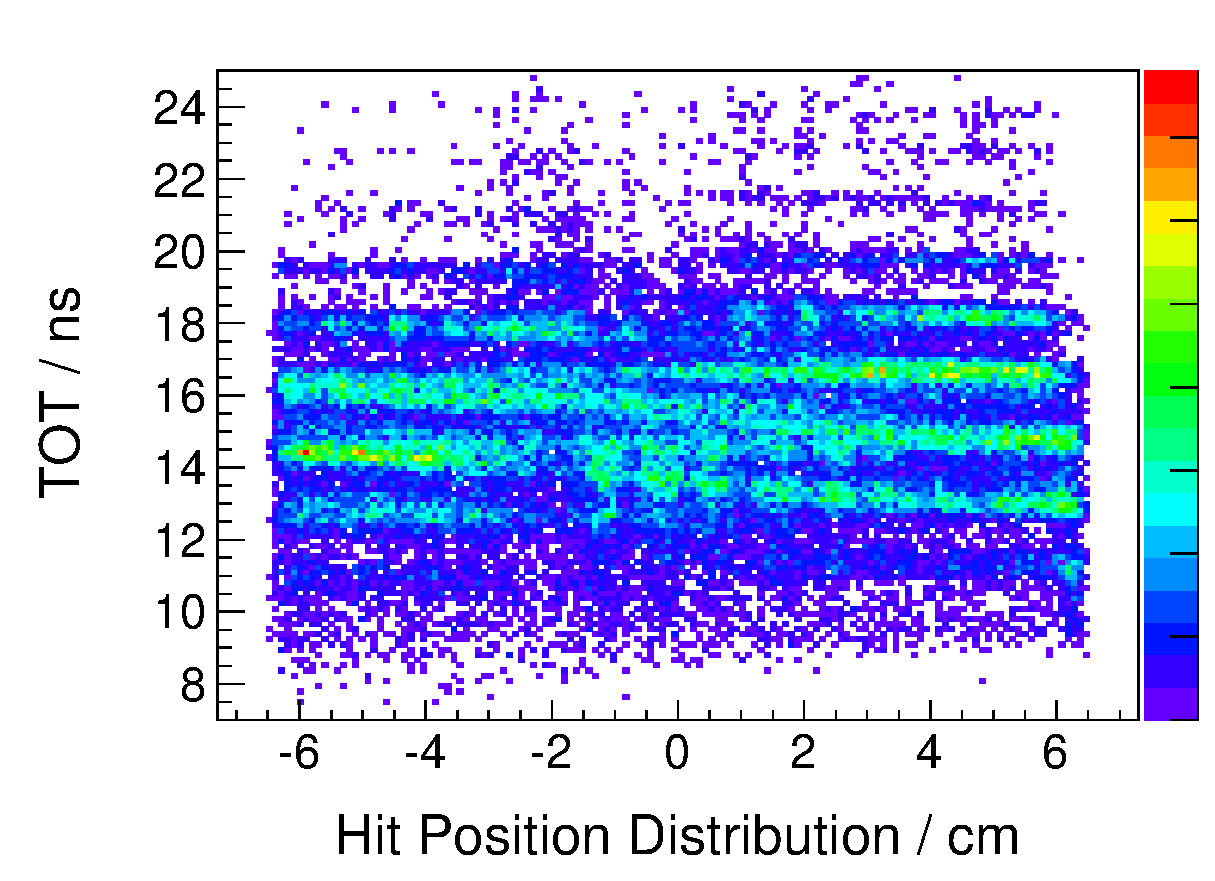
\includegraphics[width=0.9\textwidth]{chap1/left-qVSz.eps}
\subcaption{过阈时间随击中位置的分布}
\label{fig:left-qVSz}
\end{minipage}
\caption{一些原始的分布}
\label{fig:some-Diagram}
\end{figure}

%束团在对撞点发生对撞,产生的次级带电粒子的速度大小和方向在各向都是同性的。
\subsection{过阈时间和反射问题}
刻度的主要内容包括:信号在读数条的传播时间项,过阈时间的修正项。

其中信号在读数条的传播时间和信号在读数条的击中位置以及信号在读数条的等效传播速度有关。对于MRPC的每条读数条而言,长度以及工艺上的差别,导致信号在每个读数条的等效速度不尽相同,因此需要分别对每条读数条进行离线刻度。

\begin{figure}[!h]
\begin{minipage}[!h]{0.5\linewidth}
%\centering
\includegraphics[width=0.8\textwidth]{chap1/TOT.png}
\subcaption{过阈时间~\cite{Shao:2009aa}~}
\label{fig:TOT}
\end{minipage}
\hfill
\begin{minipage}[!h]{0.5\linewidth}
%\centering
\includegraphics[width=0.9\textwidth]{chap1/reflection.png}
\subcaption{反射问题}
\label{fig:reflection}
\end{minipage}%
\caption{反射问题和过阈时间}
\end{figure}
信号在读数条的传播时间项如图~\ref{fig:left-tVSz}~所示,近似是一个线性的关系。预估采用低阶多项式即可完成修正。而过阈时间修正项如图~\ref{fig:left-tVSq}~所示,可以看出时间对TOT的分布存在折线关系,分布复杂,需要分析这种折线分布背后的产生的机制。采用合适的方式处理这种关系。
图~\ref{fig:TOT}~是信号的过阈时间。对于一定的阈值,幅度大小不同的信号,对应的过阈时间不同。信号幅度越大,过阈时间也就越大。
图~\ref{fig:left-q}~中~TOT~的多峰来自于反射。
图~\ref{fig:reflection}~是~MRPC~读数条的反射问题,分为近端反射和远端反射。由于读数条本身较短,反射信号只是比真实信号时间晚不到1ns,这样导致反射信号和原来的真实信号叠加。测量的~TOT~也就变大了。
正是由于过阈时间和反射问题的存在,导致时间对~TOT~的分布复杂。对时间和~TOT~的关系的研究也刻度研究的重点和难点部分。

\section{小结}
本章首先介绍了原来的端盖闪烁体~TOF~的时间分辨等性能,由于时间分辨达不到~BESIII~实验高精度测量的要求,端盖~TOF~在~2015~年完成了升级改造,换成了时间分辨更好的~MRPC~探测器。~MRPC~探测器作为一种新型的飞行时间探测器,具有时间分辨好,探测效率高,造价便宜等优势。之后介绍了BESIII实验的MRPC的结构。~BESIII~的离线数据处理和分析系统可以处理包括模拟、刻度、重建和物理分析等一系列的物理问题,其中~BOSS~是整个离线软件的核心。然后介绍了事例起始时间的重建,MDC~的径迹外推,以及~TOF~的离线数据重建过程。最后介绍了~MRPC~端盖TOF的一些原始分布以及刻度的主要内容,由于反射的原因,导致时间和TOT的关系分布复杂。过阈时间的修正是刻度的重点和难点部分。







